\documentclass[11pt]{article}

\usepackage[margin=1in]{geometry}
\usepackage[T1]{fontenc}
\usepackage[utf8]{inputenc}
\usepackage{lmodern}
\usepackage{microtype}
\usepackage{amsmath,amssymb,amsthm,mathtools}
\usepackage{bm}
\usepackage{booktabs,array,longtable}
\usepackage{hyperref}
\usepackage{xcolor}
\usepackage[most]{tcolorbox}
\usepackage{tikz}
\usepackage{pgfplots}
\usepackage{pgfplotstable}
\usepackage{tikz-3dplot}
\usepackage{enumitem}
\usepackage{caption}
\usepackage{float}
\usepackage{fancyhdr}
\usepackage{titlesec}

\pgfplotsset{compat=1.18}
\usepgfplotslibrary{fillbetween}
\usetikzlibrary{arrows.meta,calc,intersections,patterns,decorations.pathreplacing,positioning,3d,backgrounds}

\hypersetup{
  colorlinks=true,
  linkcolor=blue!60!black,
  urlcolor=blue!60!black,
  citecolor=blue!60!black,
  pdftitle={Chapter 7. Limits and Continuity in Several Variables}
}

\setlength{\headheight}{14pt}
\setlength{\parindent}{0pt}
\setlength{\parskip}{0.65em}
\setlist[itemize]{topsep=2pt,itemsep=2pt}
\setlist[enumerate]{topsep=2pt,itemsep=2pt}

\titleformat{\section}{\large\bfseries}{\thesection}{0.6em}{}
\titleformat{\subsection}{\normalsize\bfseries}{\thesubsection}{0.6em}{}

\pagestyle{fancy}
\fancyhf{}
\lhead{Chapter 7. Limits and Continuity}
\rhead{\thepage}
\renewcommand{\headrulewidth}{0.4pt}

\newtcolorbox{chapteroverviewbox}{
  colback=blue!4,
  colframe=blue!50!black,
  boxrule=0.7pt,
  arc=2mm,
  left=2mm,right=2mm,top=1mm,bottom=1mm
}

\newtcolorbox{goalbox}{
  colback=green!4,
  colframe=green!45!black,
  title=Learning goals,
  fonttitle=\bfseries,
  boxrule=0.7pt,
  arc=2mm
}

\newtcolorbox{notebox}[1][]{
  colback=blue!3,
  colframe=blue!50!black,
  fonttitle=\bfseries,
  title=#1,
  boxrule=0.7pt,
  arc=2mm
}

\newtcolorbox{importantbox}[1][]{
  colback=red!3,
  colframe=red!65!black,
  fonttitle=\bfseries,
  title=#1,
  boxrule=0.7pt,
  arc=2mm
}

\newtcolorbox{tipbox}[1][]{
  colback=green!3,
  colframe=green!45!black,
  fonttitle=\bfseries,
  title=#1,
  boxrule=0.7pt,
  arc=2mm
}

\newtcolorbox{warningbox}[1][]{
  colback=yellow!8,
  colframe=orange!75!black,
  fonttitle=\bfseries,
  title=#1,
  boxrule=0.7pt,
  arc=2mm
}

\newtcbtheorem[number within=section]{workedexample}{Example}{
  enhanced,
  breakable,
  colback=white,
  colframe=blue!60!black,
  colbacktitle=blue!60!black,
  fonttitle=\bfseries,
  boxrule=0.7pt,
  arc=1.5mm,
  left=2mm,right=2mm,top=1mm,bottom=1mm
}{ex}

\newcommand{\R}{\mathbb R}
\newcommand{\dd}{\,d}
\newcommand{\norm}[1]{\left\lVert #1\right\rVert}
\newcommand{\abs}[1]{\left\lvert #1\right\rvert}

\begin{document}

\begin{center}
  {\LARGE\bfseries Chapter 7. Limits and Continuity in Several Variables\par}
  \vspace{0.3em}
  {\large Path dependence, continuity, and local stability\par}
\end{center}

\begin{chapteroverviewbox}
In single-variable calculus, the limit
\[
\lim_{x\to a} f(x)
\]
asks what happens as $x$ approaches $a$ from the left and from the right. In multivariable calculus, the limit
\[
\lim_{(x,y)\to(a,b)} f(x,y)
\]
asks what happens as the point $(x,y)$ approaches $(a,b)$ from every possible direction and along every possible path. This is the first major conceptual difference between single-variable and multivariable calculus.

This chapter is about learning how to decide when a multivariable limit exists, when it fails to exist, and why continuity is the local stability condition that makes differentiation and integration behave well.
\end{chapteroverviewbox}

\begin{notebox}[Connection]
This chapter develops limits and continuity of functions of several variables, including the distance-based definition, path tests, examples such as $\frac{x^2-y^2}{x^2+y^2}$ and $\frac{xy^2}{x^2+y^4}$, and continuous examples such as $e^{-xy}\sin(x+y)$ and $\frac{\sin(x^2+y^2)}{x^2+y^2}$.
\end{notebox}

\begin{goalbox}
After studying this chapter, you should be able to:
\begin{enumerate}
  \item explain the meaning of $\lim_{(x,y)\to(a,b)} f(x,y)=L$;
  \item use direct substitution when continuity applies;
  \item show that a limit does not exist by finding two paths with different limiting values;
  \item understand why checking only lines is sometimes not enough;
  \item prove simple limits using estimates, polar coordinates, and the squeeze theorem;
  \item define continuity for functions of several variables;
  \item identify common sources of discontinuity;
  \item use numerical and graphical evidence responsibly;
  \item connect continuity to stability in statistics, data science, and machine learning.
\end{enumerate}
\end{goalbox}

\section{Why multivariable limits are different}

A single-variable limit has only two basic directions of approach:
\[
x\to a^- \qquad \text{and} \qquad x\to a^+.
\]
A two-variable limit has infinitely many possible approaches:
\[
(x,y)\to(a,b).
\]
The point $(x,y)$ can approach $(a,b)$ along a horizontal line, a vertical line, a slanted line, a parabola, a spiral, or a more complicated curve. For the limit to exist, \emph{all paths must lead to the same value}.

\begin{importantbox}[Core idea]
To prove a multivariable limit exists, we must control all possible approaches. To prove a multivariable limit does not exist, it is enough to find two approaches that give different answers.
\end{importantbox}

A useful analogy is hiking toward the summit of a mountain. If all trails leading to the summit approach the same height, the height has a well-defined limit. If different trails approach different heights near the same map location, then the surface does not have a well-defined limiting height there.

\begin{figure}[H]
\centering
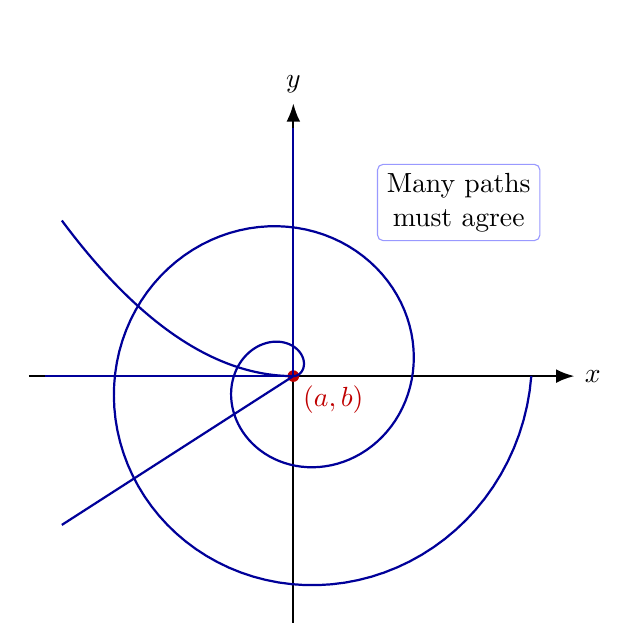
\begin{tikzpicture}[scale=1.05]
  \draw[-Latex,thick] (-3.2,0)--(3.4,0) node[right] {$x$};
  \draw[-Latex,thick] (0,-3.1)--(0,3.3) node[above] {$y$};
  \fill[red!75!black] (0,0) circle (2pt) node[below right] {$(a,b)$};
  \draw[blue!60!black,thick] (-3,0)--(0,0);
  \draw[blue!60!black,thick] (0,3)--(0,0);
  \draw[blue!60!black,thick] (-2.8,-1.8)--(0,0);
  \draw[blue!60!black,thick,domain=-2.8:0,samples=80] plot (\x,{0.24*(\x)^2});
  \draw[blue!60!black,thick,domain=0:720,samples=200,variable=\t] plot ({0.004*\t*cos(\t)},{0.004*\t*sin(\t)});
  \node[align=center,fill=white,draw=blue!40,rounded corners=2pt] at (2.0,2.1) {Many paths\\must agree};
\end{tikzpicture}
\caption{In two variables, a point can approach the target along infinitely many paths.}
\end{figure}

\section{The formal definition}

Let $f$ be a function of two variables whose domain contains points arbitrarily close to $(a,b)$. We write
\[
\lim_{(x,y)\to(a,b)} f(x,y)=L
\]
if the values $f(x,y)$ become arbitrarily close to $L$ whenever $(x,y)$ is sufficiently close to $(a,b)$, but not equal to $(a,b)$.

Using distance, this means:
\[
0<\sqrt{(x-a)^2+(y-b)^2}<\delta
\quad \Longrightarrow \quad
\abs{f(x,y)-L}<\varepsilon.
\]
Here $\varepsilon$ measures closeness in output, and $\delta$ measures closeness in input.

\begin{tipbox}[Practical interpretation]
The formal definition says that the output can be forced close to $L$ by taking the input point close enough to $(a,b)$, regardless of the direction of approach.
\end{tipbox}

The same definition works in $\R^n$. If $x=(x_1,\ldots,x_n)$ and $a=(a_1,\ldots,a_n)$, then
\[
\norm{x-a}=\sqrt{(x_1-a_1)^2+\cdots+(x_n-a_n)^2}.
\]
Then
\[
\lim_{x\to a} f(x)=L
\]
means that $f(x)$ is close to $L$ whenever $\norm{x-a}$ is small and nonzero.

\begin{figure}[H]
\centering
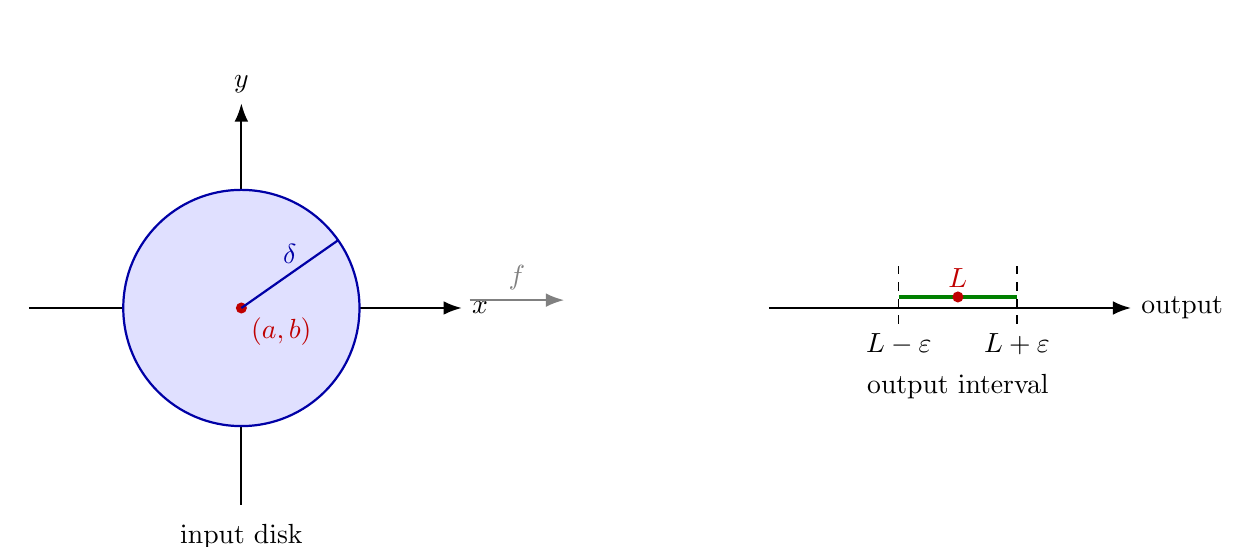
\begin{tikzpicture}[scale=1.0]
  \begin{scope}
    \draw[-Latex,thick] (-2.7,0)--(2.8,0) node[right] {$x$};
    \draw[-Latex,thick] (0,-2.5)--(0,2.6) node[above] {$y$};
    \fill[blue!12] (0,0) circle (1.5);
    \draw[blue!65!black,thick] (0,0) circle (1.5);
    \fill[red!75!black] (0,0) circle (2pt) node[below right] {$(a,b)$};
    \draw[blue!65!black,thick] (0,0)--({1.5*cos(35)},{1.5*sin(35)}) node[midway,above] {$\delta$};
    \node[align=center] at (0,-2.9) {input disk};
  \end{scope}
  \begin{scope}[xshift=7.1cm]
    \draw[-Latex,thick] (-0.4,0)--(4.2,0) node[right] {output};
    \draw[green!50!black,very thick] (1.25,0.14)--(2.75,0.14);
    \draw[dashed] (1.25,-0.2)--(1.25,0.55);
    \draw[dashed] (2.75,-0.2)--(2.75,0.55);
    \fill[red!75!black] (2,0.14) circle (2pt) node[above] {$L$};
    \node[below] at (1.25,-0.2) {$L-\varepsilon$};
    \node[below] at (2.75,-0.2) {$L+\varepsilon$};
    \node[align=center] at (2,-1.0) {output interval};
  \end{scope}
  \draw[-Latex,thick,gray] (2.9,0.1)--(4.1,0.1) node[midway,above] {$f$};
\end{tikzpicture}
\caption{The $\varepsilon$-$\delta$ definition controls all points in a small punctured disk around the input point.}
\end{figure}

\section{Easy limits by continuity}

Many limits are easy because the function is continuous. Polynomials, exponential functions, trigonometric functions, and compositions of continuous functions are continuous wherever they are defined.

\begin{workedexample}{Direct substitution}{directsub}
Evaluate
\[
\lim_{(x,y)\to(0,0)} e^{-xy}\sin(x+y).
\]
Both $e^{-xy}$ and $\sin(x+y)$ are continuous, so their product is continuous. Therefore the limit is obtained by substitution:
\[
\lim_{(x,y)\to(0,0)} e^{-xy}\sin(x+y)=e^0\sin(0)=0.
\]
\end{workedexample}

\begin{workedexample}{A rational function at a regular point}{rationalregular}
Evaluate
\[
\lim_{(x,y)\to(1,2)} \frac{x+y^2}{x^2-y^2}.
\]
The denominator at $(1,2)$ is
\[
1^2-2^2=-3\ne 0.
\]
So the function is continuous at $(1,2)$, and
\[
\lim_{(x,y)\to(1,2)} \frac{x+y^2}{x^2-y^2}
=
\frac{1+2^2}{1^2-2^2}
=-\frac{5}{3}.
\]
\end{workedexample}

\begin{notebox}[When substitution works]
If a formula is built from continuous operations and is defined at the target point, substitution is usually the first method to try.
\end{notebox}

\section{Path tests for nonexistence}

To show a limit does not exist, find two paths approaching the same point that give different limiting values.

\begin{workedexample}{A classic path-dependent limit}{pathdep}
Consider
\[
f(x,y)=\frac{x^2-y^2}{x^2+y^2}.
\]
Along the path $y=0$,
\[
f(x,0)=\frac{x^2}{x^2}=1,
\]
so $\lim_{x\to0} f(x,0)=1$. Along the path $x=0$,
\[
f(0,y)=\frac{-y^2}{y^2}=-1,
\]
so $\lim_{y\to0} f(0,y)=-1$. The two paths give different values. Therefore
\[
\lim_{(x,y)\to(0,0)} \frac{x^2-y^2}{x^2+y^2}
\]
does not exist.
\end{workedexample}

Along a general line $y=mx$ with $x\ne0$,
\[
f(x,mx)=\frac{x^2-m^2x^2}{x^2+m^2x^2}
=
\frac{1-m^2}{1+m^2}.
\]
The result depends on $m$, the slope of the path. That is a strong sign that the full two-variable limit does not exist.

\begin{figure}[H]
\centering
\begin{minipage}{0.46\textwidth}
\centering
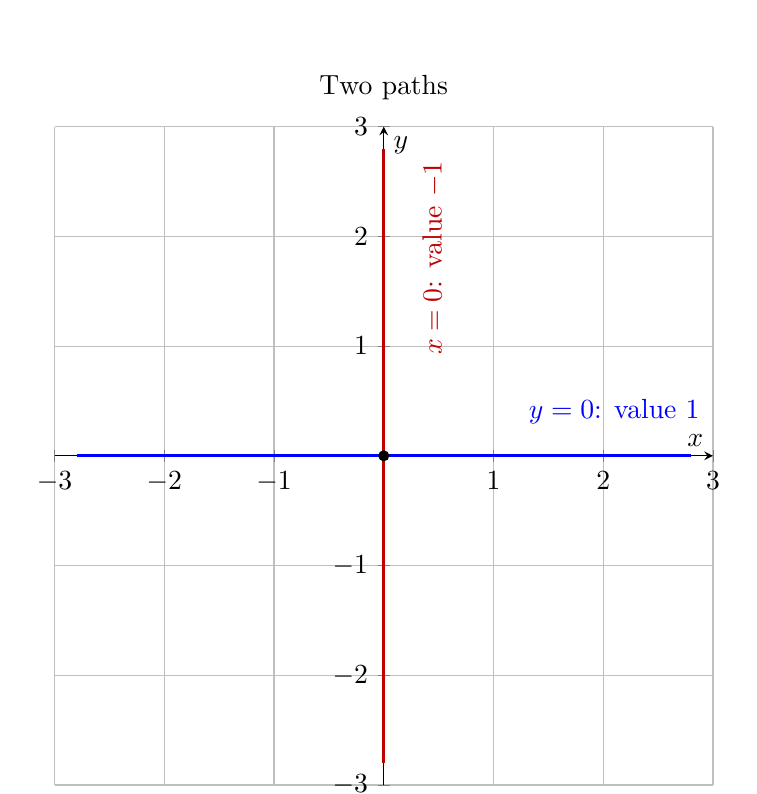
\begin{tikzpicture}
\begin{axis}[
  width=\textwidth,
  height=0.82\textwidth,
  xmin=-3,xmax=3,ymin=-3,ymax=3,
  axis equal image,
  axis lines=middle,
  xlabel={$x$},ylabel={$y$},
  grid=both,
  title={Two paths}
]
\addplot[very thick,blue,domain=-2.8:2.8] {0};
\addplot[very thick,red!75!black] coordinates {(0,-2.8) (0,2.8)};
\fill (axis cs:0,0) circle (2pt);
\node[blue] at (axis cs:2.1,0.4) {$y=0$: value $1$};
\node[red!75!black,rotate=90] at (axis cs:0.45,1.8) {$x=0$: value $-1$};
\end{axis}
\end{tikzpicture}
\end{minipage}\hfill
\begin{minipage}{0.5\textwidth}
\centering
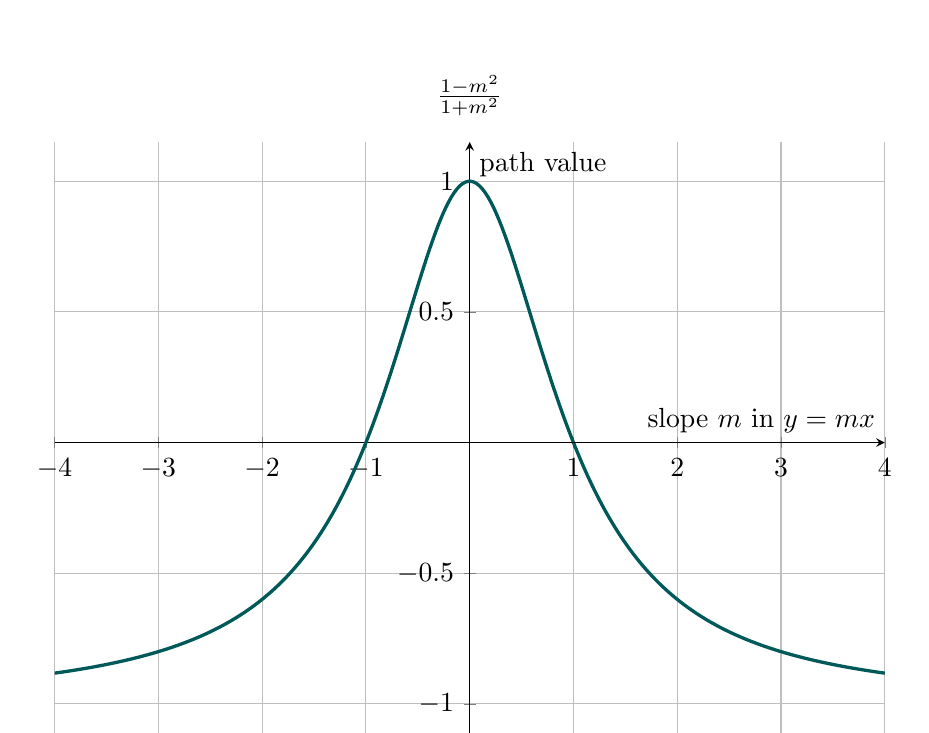
\begin{tikzpicture}
\begin{axis}[
  width=\textwidth,
  height=0.76\textwidth,
  xmin=-4,xmax=4,ymin=-1.15,ymax=1.15,
  axis lines=middle,
  xlabel={slope $m$ in $y=mx$},
  ylabel={path value},
  grid=both,
  title={$\frac{1-m^2}{1+m^2}$}
]
\addplot[very thick,teal!70!black,domain=-4:4,samples=300] {(1-x^2)/(1+x^2)};
\addplot[dashed] coordinates {(-4,0) (4,0)};
\end{axis}
\end{tikzpicture}
\end{minipage}
\caption{Different straight-line paths give different limiting values for $f(x,y)=\frac{x^2-y^2}{x^2+y^2}$.}
\end{figure}

\begin{figure}[H]
\centering
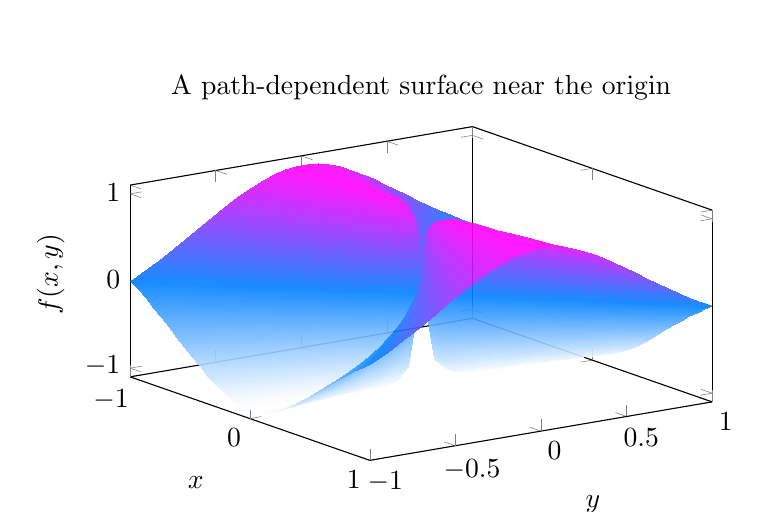
\begin{tikzpicture}
\begin{axis}[
  width=0.74\textwidth,
  height=0.48\textwidth,
  view={55}{28},
  xlabel={$x$},ylabel={$y$},zlabel={$f(x,y)$},
  domain=-1:1,y domain=-1:1,
  samples=32,samples y=32,
  zmin=-1.1,zmax=1.1,
  colormap/cool,
  title={A path-dependent surface near the origin}
]
\addplot3[surf,shader=interp,opacity=0.9] {(x^2-y^2)/(x^2+y^2)};
\end{axis}
\end{tikzpicture}
\caption{Near the origin, the surface approaches different heights from different directions.}
\end{figure}

\section{Checking only lines is not enough}

Sometimes every straight-line path gives the same value, but the limit still does not exist. This is one of the most important warnings in multivariable calculus.

\begin{workedexample}{Lines are misleading}{linesnotenough}
Consider
\[
g(x,y)=\frac{xy^2}{x^2+y^4}.
\]
Along a straight line $y=mx$,
\[
g(x,mx)=\frac{x(m^2x^2)}{x^2+m^4x^4}
=
\frac{m^2x}{1+m^4x^2}\to0.
\]
So every line $y=mx$ gives limiting value $0$.

But along the curved path $x=y^2$,
\[
g(y^2,y)=\frac{y^2y^2}{(y^2)^2+y^4}=\frac{y^4}{2y^4}=\frac12.
\]
Therefore the full limit does not exist.
\end{workedexample}

\begin{figure}[H]
\centering
\begin{minipage}{0.45\textwidth}
\centering
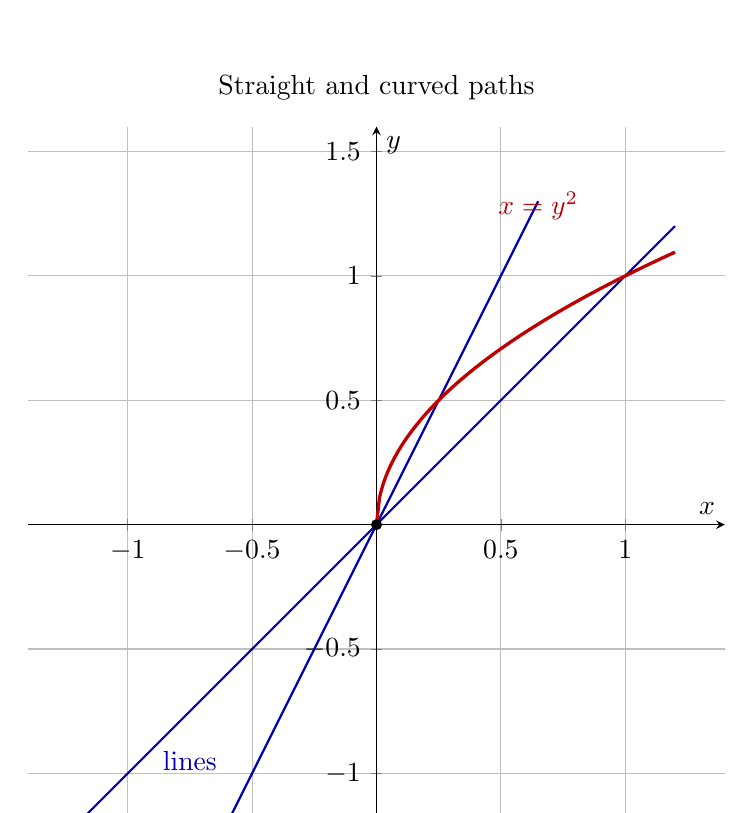
\begin{tikzpicture}
\begin{axis}[
  width=\textwidth,
  height=0.86\textwidth,
  xmin=-1.4,xmax=1.4,ymin=-1.2,ymax=1.6,
  axis equal image,
  axis lines=middle,
  xlabel={$x$},ylabel={$y$},
  grid=both,
  title={Straight and curved paths}
]
\addplot[blue!65!black,thick,domain=-1.2:1.2] {x};
\addplot[blue!65!black,thick,domain=-0.65:0.65] {2*x};
\addplot[red!75!black,very thick,domain=0:1.2,samples=100] {sqrt(x)};
\node[blue!65!black] at (axis cs:-0.75,-0.95) {lines};
\node[red!75!black] at (axis cs:0.65,1.28) {$x=y^2$};
\fill (axis cs:0,0) circle (2pt);
\end{axis}
\end{tikzpicture}
\end{minipage}\hfill
\begin{minipage}{0.52\textwidth}
\centering
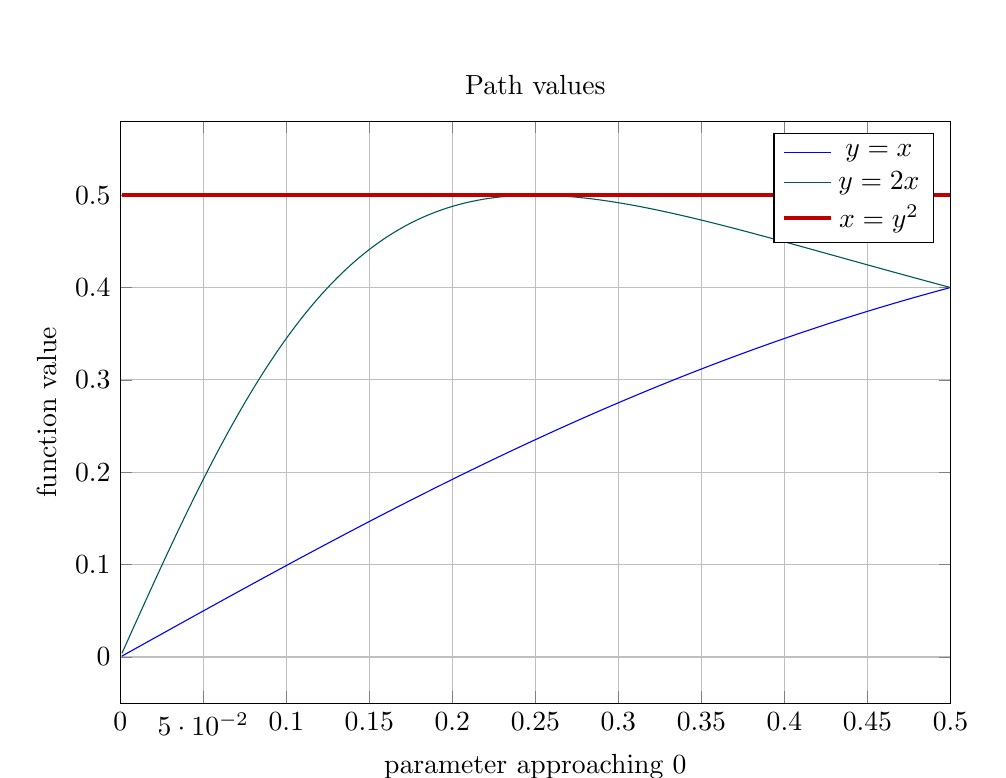
\begin{tikzpicture}
\begin{axis}[
  width=\textwidth,
  height=0.74\textwidth,
  xmin=0,xmax=0.5,ymin=-0.05,ymax=0.58,
  xlabel={parameter approaching $0$},
  ylabel={function value},
  grid=both,
  legend style={at={(0.98,0.98)},anchor=north east,fill=white},
  title={Path values}
]
\addplot[blue,domain=0.001:0.5,samples=200] {x/(1+x^2)};
\addlegendentry{$y=x$}
\addplot[teal!70!black,domain=0.001:0.5,samples=200] {4*x/(1+16*x^2)};
\addlegendentry{$y=2x$}
\addplot[red!75!black,very thick,domain=0.001:0.5,samples=2] {0.5};
\addlegendentry{$x=y^2$}
\end{axis}
\end{tikzpicture}
\end{minipage}
\caption{Line paths can all approach zero while a curved path approaches a different value.}
\end{figure}

\begin{warningbox}[Common mistake]
Showing that several paths give the same value does not prove a limit exists. It only provides evidence. To prove existence, we need an argument that controls all paths.
\end{warningbox}

\section{Proving limits with estimates}

To prove that a limit exists, we often use inequalities. The idea is to bound the complicated expression by something simpler that goes to zero.

A common strategy near $(0,0)$ is to use
\[
r=\sqrt{x^2+y^2}.
\]
Then
\[
\abs{x}\le r, \qquad \abs{y}\le r.
\]
If we can show
\[
\abs{f(x,y)-L}\le C r^p
\]
for constants $C>0$ and $p>0$, then $f(x,y)\to L$ as $(x,y)\to(0,0)$.

\begin{workedexample}{A squeeze theorem proof}{squeeze}
Show that
\[
\lim_{(x,y)\to(0,0)} \frac{x^2y}{x^2+y^2}=0.
\]
For $(x,y)\ne(0,0)$,
\[
\left|\frac{x^2y}{x^2+y^2}\right|
=
\frac{\abs{x}^2\abs{y}}{x^2+y^2}.
\]
Since $x^2\le x^2+y^2$, we have
\[
\frac{\abs{x}^2}{x^2+y^2}\le1.
\]
Therefore
\[
\left|\frac{x^2y}{x^2+y^2}\right|\le \abs{y}.
\]
As $(x,y)\to(0,0)$, we have $\abs{y}\to0$. By the squeeze theorem,
\[
\lim_{(x,y)\to(0,0)} \frac{x^2y}{x^2+y^2}=0.
\]
\end{workedexample}

\begin{figure}[H]
\centering
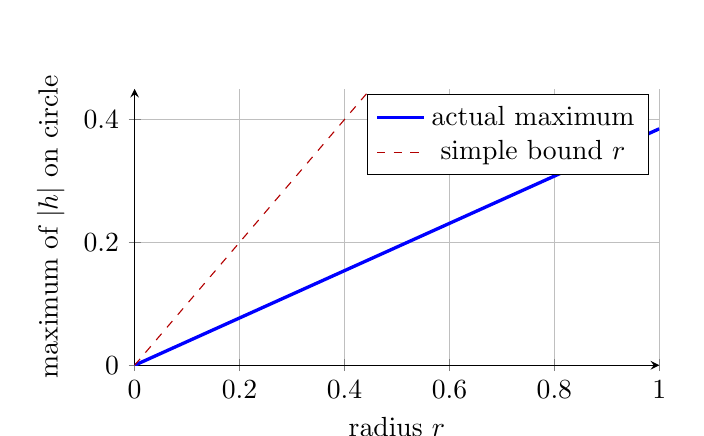
\begin{tikzpicture}
\begin{axis}[
  width=0.68\textwidth,
  height=0.42\textwidth,
  xmin=0,xmax=1,ymin=0,ymax=0.45,
  axis lines=left,
  xlabel={radius $r$},
  ylabel={maximum of $|h|$ on circle},
  grid=both,
  legend style={at={(0.98,0.98)},anchor=north east,fill=white}
]
\addplot[very thick,blue,domain=0:1,samples=100] {0.3849*x};
\addlegendentry{actual maximum}
\addplot[red!70!black,dashed,domain=0:1,samples=100] {x};
\addlegendentry{simple bound $r$}
\end{axis}
\end{tikzpicture}
\caption{For $h(x,y)=\frac{x^2y}{x^2+y^2}$, the maximum absolute value on circles of radius $r$ decreases linearly toward zero.}
\end{figure}

\section{Polar coordinates as a limit tool}

For limits at the origin in the plane, polar coordinates are often useful:
\[
x=r\cos\theta, \qquad y=r\sin\theta.
\]
Then $(x,y)\to(0,0)$ means $r\to0$. The angle $\theta$ may change in any way. If the expression becomes something that goes to $L$ independently of $\theta$, then the limit is $L$.

\begin{workedexample}{A polar-coordinate proof}{polarproof}
Show that
\[
\lim_{(x,y)\to(0,0)} \frac{xy}{\sqrt{x^2+y^2}}=0.
\]
Using $x=r\cos\theta$ and $y=r\sin\theta$,
\[
\frac{xy}{\sqrt{x^2+y^2}}
=
\frac{r^2\cos\theta\sin\theta}{r}
=
r\cos\theta\sin\theta.
\]
Since $\abs{\cos\theta\sin\theta}\le1$,
\[
\abs{r\cos\theta\sin\theta}\le r.
\]
As $r\to0$, this tends to $0$. Therefore
\[
\lim_{(x,y)\to(0,0)} \frac{xy}{\sqrt{x^2+y^2}}=0.
\]
\end{workedexample}

\begin{figure}[H]
\centering
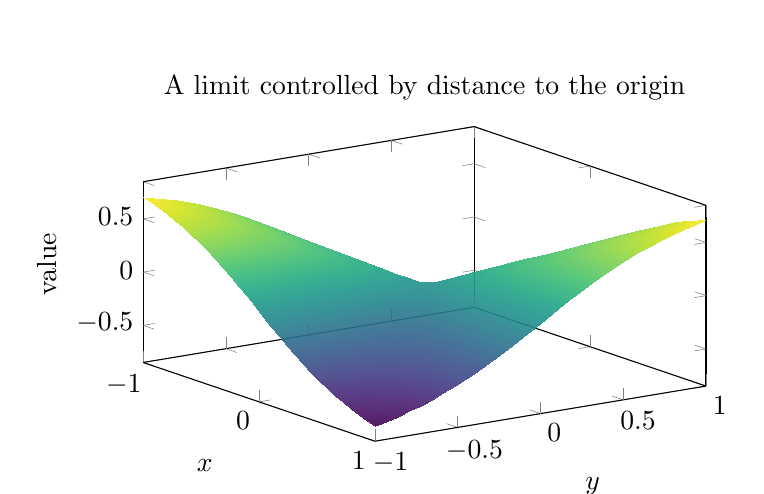
\begin{tikzpicture}
\begin{axis}[
  width=0.72\textwidth,
  height=0.46\textwidth,
  view={55}{28},
  xlabel={$x$},ylabel={$y$},zlabel={value},
  domain=-1:1,y domain=-1:1,
  samples=30,samples y=30,
  colormap/viridis,
  title={A limit controlled by distance to the origin}
]
\addplot3[surf,shader=interp,opacity=0.9] {x*y/sqrt(x^2+y^2+0.0005)};
\end{axis}
\end{tikzpicture}
\caption{The polar form $r\cos\theta\sin\theta$ is controlled by the radius $r$.}
\end{figure}

\section{A removable discontinuity}

Consider
\[
q(x,y)=\frac{\sin(x^2+y^2)}{x^2+y^2}.
\]
The expression is undefined at $(0,0)$, but the limit exists. Let
\[
u=x^2+y^2.
\]
As $(x,y)\to(0,0)$, we have $u\to0^+$. Therefore
\[
\lim_{(x,y)\to(0,0)} \frac{\sin(x^2+y^2)}{x^2+y^2}
=
\lim_{u\to0^+}\frac{\sin u}{u}=1.
\]
The function is not continuous at the origin because it is not defined there. But we can make it continuous by defining
\[
q(0,0)=1.
\]
This is called a \emph{removable discontinuity}.

\begin{figure}[H]
\centering
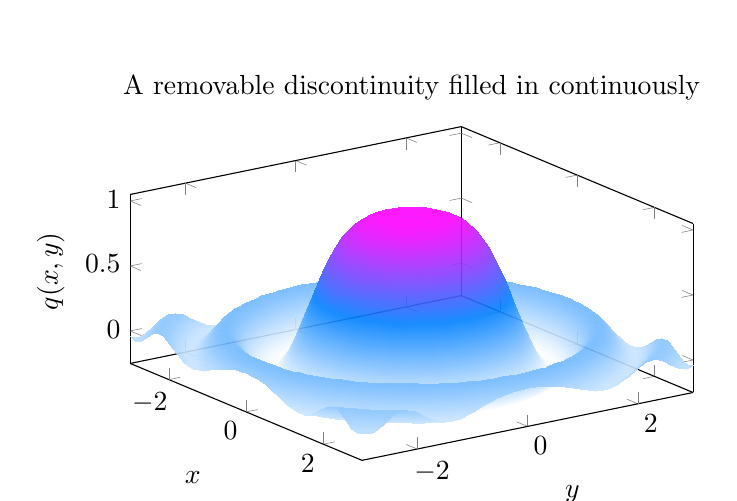
\begin{tikzpicture}
\begin{axis}[
  width=0.72\textwidth,
  height=0.48\textwidth,
  view={55}{35},
  xlabel={$x$},ylabel={$y$},zlabel={$q(x,y)$},
  domain=-3:3,y domain=-3:3,
  samples=45,samples y=45,
  zmin=-0.25,zmax=1.05,
  colormap/cool,
  title={A removable discontinuity filled in continuously}
]
\addplot3[surf,shader=interp,opacity=0.9] {sin(deg(x^2+y^2))/(x^2+y^2+0.0001)};
\end{axis}
\end{tikzpicture}
\caption{The function $\frac{\sin(x^2+y^2)}{x^2+y^2}$ has limiting value $1$ at the origin.}
\end{figure}

\section{Continuity in several variables}

A function $f(x,y)$ is \emph{continuous at} $(a,b)$ if
\[
\lim_{(x,y)\to(a,b)} f(x,y)=f(a,b).
\]
This requires three things:
\begin{enumerate}
  \item $f(a,b)$ is defined;
  \item $\lim_{(x,y)\to(a,b)} f(x,y)$ exists;
  \item the limit equals the function value.
\end{enumerate}
A function is continuous on a region $D$ if it is continuous at every point of $D$.

\subsection*{Common sources of discontinuity}

\begin{center}
\begin{tabular}{@{}>{\raggedright\arraybackslash}p{0.22\textwidth}>{\raggedright\arraybackslash}p{0.25\textwidth}>{\raggedright\arraybackslash}p{0.4\textwidth}@{}}
\toprule
Source & Example & What can go wrong? \\
\midrule
Denominator zero & $\dfrac{1}{x^2+y^2}$ & infinite blow-up near the origin \\
Path dependence & $\dfrac{x^2-y^2}{x^2+y^2}$ & different paths give different values \\
Removable hole & $\dfrac{\sin(x^2+y^2)}{x^2+y^2}$ & formula undefined at one point, but limit exists \\
Domain boundary & $\sqrt{1-x^2-y^2}$ & function exists only on a disk \\
Piecewise rule & threshold or classifier & jump discontinuity across a boundary \\
\bottomrule
\end{tabular}
\end{center}

\begin{tipbox}[Continuity and modeling]
A continuous model changes outputs gradually when inputs are changed slightly. This is essential for numerical stability, optimization, interpolation, and sensitivity analysis.
\end{tipbox}

\section{Continuity on domains and boundaries}

Some functions are continuous on their natural domains even though the domain has a boundary. For example,
\[
f(x,y)=\sqrt{1-x^2-y^2}
\]
is defined on the disk
\[
D=\{(x,y):x^2+y^2\le1\}.
\]
It is continuous at every point of this disk relative to its domain. Near boundary points, we only approach through points in the domain.

\begin{figure}[H]
\centering
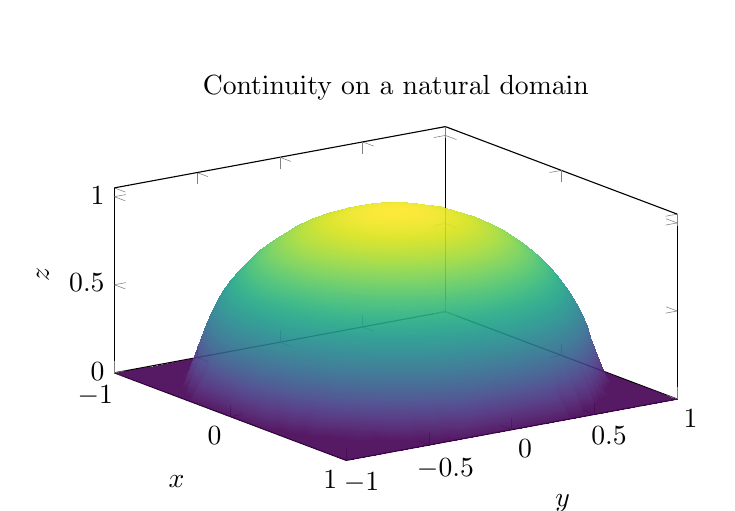
\begin{tikzpicture}
\begin{axis}[
  width=0.72\textwidth,
  height=0.48\textwidth,
  view={55}{30},
  xlabel={$x$},ylabel={$y$},zlabel={$z$},
  domain=-1:1,y domain=-1:1,
  samples=35,samples y=35,
  zmin=0,zmax=1.05,
  colormap/viridis,
  title={Continuity on a natural domain}
]
\addplot3[surf,shader=interp,opacity=0.9] {sqrt(max(0,1-x^2-y^2))};
\end{axis}
\end{tikzpicture}
\caption{The upper hemisphere is continuous on the closed disk $x^2+y^2\le1$.}
\end{figure}

This distinction matters in applications. A probability density may be defined only on a simplex, a loss function may be meaningful only on feasible parameters, and a physical model may be valid only inside a spatial region.

\section{Numerical experiments with limits}

Numerical exploration can suggest whether a limit exists, but it cannot by itself prove a limit. A computer can sample many paths, but it cannot sample all paths.

\begin{figure}[H]
\centering
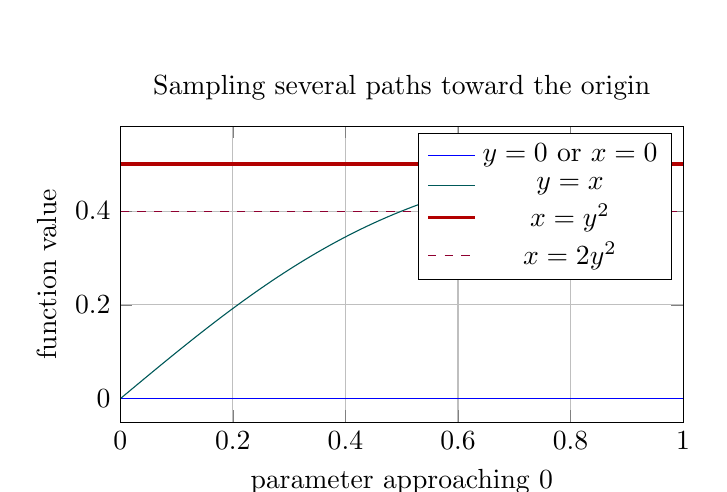
\begin{tikzpicture}
\begin{axis}[
  width=0.72\textwidth,
  height=0.44\textwidth,
  xmin=0,xmax=1,ymin=-0.05,ymax=0.58,
  xlabel={parameter approaching $0$},
  ylabel={function value},
  grid=both,
  legend style={at={(0.98,0.98)},anchor=north east,fill=white},
  title={Sampling several paths toward the origin}
]
\addplot[blue,domain=0.001:1,samples=200] {0};
\addlegendentry{$y=0$ or $x=0$}
\addplot[teal!70!black,domain=0.001:1,samples=200] {x/(1+x^2)};
\addlegendentry{$y=x$}
\addplot[red!70!black,very thick,domain=0.001:1,samples=2] {0.5};
\addlegendentry{$x=y^2$}
\addplot[purple!75!black,dashed,domain=0.001:1,samples=2] {0.4};
\addlegendentry{$x=2y^2$}
\end{axis}
\end{tikzpicture}
\caption{Numerical path sampling is useful evidence but not a proof.}
\end{figure}

\begin{warningbox}[Computational caution]
A graph can miss a narrow ridge, a sharp spike, or a curved path where behavior changes. Use computation to develop intuition, then use algebra to justify the conclusion.
\end{warningbox}

\section{Higher-dimensional continuity}

For a function
\[
f:\R^n\to\R,
\]
continuity at $a\in\R^n$ means
\[
\lim_{x\to a} f(x)=f(a).
\]
The same distance idea applies:
\[
\norm{x-a}<\delta
\quad \Longrightarrow \quad
\abs{f(x)-f(a)}<\varepsilon.
\]
For example, the squared norm function
\[
f(x)=\norm{x}^2=x_1^2+\cdots+x_n^2
\]
is continuous on $\R^n$. The logistic regression loss, least-squares loss, and many smooth neural-network losses are also continuous functions of their parameters.

\begin{workedexample}{Least-squares loss is continuous}{least-squares-cont}
Let $A$ be a fixed data matrix and $b$ a fixed response vector. Define
\[
L(w)=\norm{Aw-b}^2.
\]
This is a polynomial function of the components of $w$, so it is continuous. Small changes in $w$ cause small changes in $L(w)$. This is one reason gradient-based methods can be used to minimize least-squares loss.
\end{workedexample}

\begin{figure}[H]
\centering
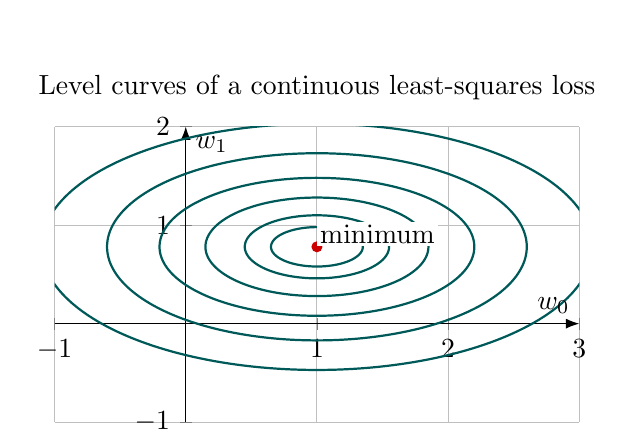
\begin{tikzpicture}
\begin{axis}[
  width=0.68\textwidth,
  height=0.44\textwidth,
  xmin=-1,xmax=3,
  ymin=-1,ymax=2,
  axis lines=middle,
  xlabel={$w_0$},ylabel={$w_1$},
  grid=both,
  axis line style={-Latex},
  title={Level curves of a continuous least-squares loss}
]
\foreach \a/\b in {0.35/0.2,0.55/0.32,0.85/0.5,1.2/0.7,1.6/0.95,2.1/1.25}{
  \addplot[domain=0:360,samples=220,teal!70!black,thick] ({1.0 + \a*cos(x)},{0.78 + \b*sin(x)});
}
\fill[red!80!black] (axis cs:1.0,0.78) circle (2pt);
\node[above right,fill=white,inner sep=1pt] at (axis cs:1.0,0.78) {minimum};
\end{axis}
\end{tikzpicture}
\caption{A least-squares loss surface is continuous and has smooth level curves.}
\end{figure}

\section{Modern applications}

\subsection*{Statistics}
In statistics, likelihood and loss functions are often functions of parameters. Continuity allows us to use local approximations, optimization methods, and asymptotic arguments. For example, if a likelihood changes continuously with parameters, then nearby parameter values produce nearby likelihood values.

\subsection*{Data science}
A data record may be a vector
\[
x=(x_1,\ldots,x_n).
\]
A prediction model may be a function
\[
f(x_1,\ldots,x_n).
\]
Continuity means that small changes in the input features produce small changes in the prediction. This is desirable for many regression models.

\subsection*{Machine learning and AI}
Training a model usually means minimizing a loss function
\[
L(\theta).
\]
Continuity of $L$ is the first requirement for meaningful optimization. Differentiability, which comes next, is stronger. A function can be continuous without being differentiable, but it cannot be differentiable without being continuous.

\begin{importantbox}[Bridge to gradients]
The next chapters build on continuity. Partial derivatives, tangent planes, gradients, and optimization all require careful local behavior near a point.
\end{importantbox}

\section{Worked examples summary}

\begin{center}
\begin{tabular}{@{}>{\raggedright\arraybackslash}p{0.22\textwidth}>{\raggedright\arraybackslash}p{0.38\textwidth}>{\raggedright\arraybackslash}p{0.28\textwidth}@{}}
\toprule
Example type & Limit & Reason \\
\midrule
Exists by continuity & $\displaystyle \lim_{(x,y)\to(1,2)}\frac{x+y^2}{x^2-y^2}=-\frac53$ & denominator is nonzero at $(1,2)$ \\
Does not exist by two paths & $\displaystyle \lim_{(x,y)\to(0,0)}\frac{x^2-y^2}{x^2+y^2}$ & $y=0$ gives $1$, while $x=0$ gives $-1$ \\
Lines are not enough & $\displaystyle \lim_{(x,y)\to(0,0)}\frac{xy^2}{x^2+y^4}$ & every line gives $0$, but $x=y^2$ gives $1/2$ \\
Exists by squeezing & $\displaystyle \lim_{(x,y)\to(0,0)}\frac{x^2y}{x^2+y^2}=0$ & absolute value is bounded above by $|y|$ \\
\bottomrule
\end{tabular}
\end{center}

\section{Practice problems}

\subsection*{Concept checks}
\begin{enumerate}
  \item Explain why multivariable limits are harder than single-variable limits.
  \item What does it mean for a function $f(x,y)$ to be continuous at $(a,b)$?
  \item Why can two different path limits prove that a limit does not exist?
  \item Why does checking only horizontal and vertical paths usually not prove that a limit exists?
  \item Explain the difference between a removable discontinuity and a path-dependent discontinuity.
\end{enumerate}

\subsection*{Computational skill problems}
\begin{enumerate}[resume]
  \item Evaluate by substitution, if possible:
  \[
  \lim_{(x,y)\to(2,-1)} (x^2y+e^{xy}).
  \]
  \item Evaluate by substitution, if possible:
  \[
  \lim_{(x,y)\to(1,1)} \frac{x^2+y^2}{x+y}.
  \]
  \item Determine whether the limit exists:
  \[
  \lim_{(x,y)\to(0,0)} \frac{x^2}{x^2+y^2}.
  \]
  \item Determine whether the limit exists:
  \[
  \lim_{(x,y)\to(0,0)} \frac{xy}{x^2+y^2}.
  \]
  \item Determine whether the limit exists:
  \[
  \lim_{(x,y)\to(0,0)} \frac{x^2y^2}{x^2+y^2}.
  \]
  \item Use polar coordinates to evaluate:
  \[
  \lim_{(x,y)\to(0,0)} \frac{x^2+y^2}{\sqrt{x^2+y^2+1}+1}.
  \]
  \item Show that
  \[
  \lim_{(x,y)\to(0,0)} \frac{x^3+y^3}{x^2+y^2}=0.
  \]
  \item Show that
  \[
  \lim_{(x,y)\to(0,0)} \frac{x^2y}{\sqrt{x^2+y^2}}=0.
  \]
  \item Determine where $f(x,y)=\dfrac{x+y}{x^2+y^2-1}$ is continuous.
  \item Determine where $g(x,y)=\sqrt{4-x^2-y^2}$ is continuous.
\end{enumerate}

\subsection*{Modeling and interpretation problems}
\begin{enumerate}[resume]
  \item A temperature function $T(x,y)$ is continuous on a city map. Explain what continuity means physically.
  \item A classifier is defined by $C(x,y)=1$ if $x+y\ge0$ and $C(x,y)=0$ if $x+y<0$. Where is this function discontinuous?
  \item Let $L(w)=\norm{Aw-b}^2$. Explain why $L$ is continuous as a function of the parameter vector $w$.
  \item Give an example of a model where discontinuity is expected or useful.
  \item Give an example of a model where continuity is important for stability.
\end{enumerate}

\subsection*{Computational practice}
\begin{enumerate}[resume]
  \item Test the paths $y=2x$, $y=-2x$, and $y=3x$ for $\frac{x^2-y^2}{x^2+y^2}$.
  \item Test several paths for a new function of your choice.
  \item Visualize the function $f(x,y)=\frac{xy}{x^2+y^2}$ near the origin.
  \item Numerically estimate the maximum of $\left|\frac{x^2y}{x^2+y^2}\right|$ on circles of radius $r$ for several values of $r$.
  \item Create a contour plot of a continuous loss function and explain why the level curves are useful.
\end{enumerate}

\section{Lab preview}

The lab for this chapter focuses on three skills:
\begin{enumerate}
  \item visualizing surfaces near singular points;
  \item sampling limits along many paths;
  \item distinguishing numerical evidence from mathematical proof.
\end{enumerate}
A useful workflow is:
\begin{enumerate}
  \item plot the surface or contour map;
  \item test simple paths such as $y=0$, $x=0$, and $y=mx$;
  \item test curved paths if needed;
  \item use algebra to prove the final result.
\end{enumerate}

\section*{Chapter summary}

A multivariable limit requires agreement along all possible paths. Direct substitution works when a function is continuous at the point. To show that a limit does not exist, it is enough to find two paths with different limiting values. To show that a limit exists, we need a path-independent argument, often using estimates, polar coordinates, or the squeeze theorem.

Continuity means that the value of a function agrees with its local limiting behavior. This idea is central not only to calculus, but also to numerical modeling, optimization, statistics, data science, and machine learning.

\end{document}
